% External (conference / seminar) version: work in progress.
% Compile with XeLaTeX (Fira fonts) from docs/slides/:
%   latexmk -xelatex matsuyama_in_space_conference.tex
% Figure: python docs/slides/make_figures.py (from the repository root).
\documentclass[10pt,aspectratio=169]{beamer}

\usetheme[progressbar=frametitle,block=fill,numbering=fraction]{metropolis}
\usepackage{appendixnumberbeamer}
\usepackage{booktabs}
\usepackage{array}
\newcolumntype{L}[1]{>{\raggedright\arraybackslash}p{#1}}
\usepackage{amsmath,amssymb,mathtools}
\usepackage{bm}
\usepackage{tikz}
\usetikzlibrary{arrows.meta,positioning,calc}
\usepackage{pgfplots}
\pgfplotsset{compat=1.18}
\usepackage{xcolor}

\definecolor{mDarkTeal}{HTML}{23373B}
\definecolor{mOrange}{HTML}{EB811B}
\definecolor{mGreen}{HTML}{14B03D}
\definecolor{mLight}{HTML}{EEEEEE}
\newcommand{\hl}[1]{\textcolor{mOrange}{#1}}
\newcommand{\mute}[1]{\textcolor{gray}{#1}}
\newcommand{\unv}{$^{\dagger}$}

\tikzset{
  box/.style={draw=mDarkTeal, rounded corners=2pt, fill=mLight, align=center,
              font=\scriptsize, inner sep=4pt, text width=#1},
  box/.default=3cm,
  hot/.style={draw=mOrange, fill=mOrange!12, line width=0.8pt},
  arr/.style={-{Stealth[length=5pt]}, mDarkTeal, line width=0.7pt},
}

\title{Matsuyama in Space}
\subtitle{Agricultural productivity, connectivity and structural transformation in Korea,
1965--85}
% TODO: authors, affiliations, venue
\author{[Authors]}
\institute{[Affiliations]}
\date{[Conference] \quad$\cdot$\quad Work in progress --- preliminary, please do not cite}

\begin{document}

\maketitle

% =====================================================================
\begin{frame}{Motivation}
  \begin{columns}[T]
    \begin{column}{0.57\textwidth}
      Korea, 1965--85: one of the fastest structural transformations on record.
      \vspace{0.4em}

      \scriptsize
      \begin{tabular}{@{}lll@{}}
        \toprule
        & $\sim$1960/65 & $\sim$1980/90 \\
        \midrule
        Real GDP per capita & 1 & $\times$4 (1985)\unv \\
        Agriculture, employment share & 59\% (1965)\unv & 25\% (1985)\unv \\
        Manufacturing, VA share & 15\% (1965) & 30\% (1985) \\
        Urban population share & 28\% (1960) & 57\% (1980), 74\% (1990) \\
        Farm household population & $\sim$14m & $<$6m (1990) \\
        \bottomrule
      \end{tabular}\\[0.3em]
      \tiny Sources: World Bank WDI; national statistics. \unv{} approximate, being updated
      from primary sources.
    \end{column}
    \begin{column}{0.39\textwidth}
      \small
      \begin{itemize}
        \item Poverty was concentrated in the \hl{countryside}. The transformation is a
              story about where farm labour went, and why.
        \item At the same time: industrial parks, an expressway network, irrigation,
              high-yield rice, and a closed, policy-priced rice market.
        \item Standard question: does farm productivity growth \emph{push} labour into
              industry, or \emph{anchor} it on the farm?
      \end{itemize}
    \end{column}
  \end{columns}
\end{frame}

\begin{frame}{This paper}
  \begin{block}{Question}
    When agricultural productivity rises, does a place \hl{commercialise} its farming or
    \hl{release} farm labour into non-farm work and migration --- and how does the answer
    depend on its connections to crop markets and to non-farm jobs?
  \end{block}
  \small
  \textbf{What we do}
  \begin{enumerate}
    \item A \textbf{spatial general-equilibrium model} of structural transformation:
          non-homothetic demand, migration nested with occupation choice, protected rice,
          import-competing grains, labour-saving mechanisation.
    \item A \textbf{baseline that reproduces history}: calibrated to Korea's 1965--85
          transformation, with later urbanisation generated by the model.
    \item A \textbf{township panel} (1960--90, annual; being digitised) and quasi-experimental
          designs (reservoirs, road paving) to discipline the mechanism.
  \end{enumerate}
\end{frame}

\begin{frame}{Preview of results (preliminary)}
  \begin{itemize}
    \item The sign of the farm-employment response to a farm productivity shock is governed by
          two distinct access margins, which connectivity moves \emph{together}.
    \item The baseline reproduces fourfold growth, a 38-point fall in farm employment and
          urbanisation from 32\% to 63\% through Engel effects, grain import competition
          and migration.
    \item Occupation wedges generate an agricultural productivity gap that \hl{widens}
          during the transformation.
    \item Companion reduced-form evidence: the same road-access shock releases labour near
          industrial parks and retains it in remote townships.
  \end{itemize}
  \vspace{0.5em}
  \begin{alertblock}{Contribution}
    Separately identify farm productivity shocks, industrial labour-demand shocks and
    connectivity, and show where their interaction produces commercialisation versus
    labour release --- then aggregate it in general equilibrium.
  \end{alertblock}
\end{frame}

\begin{frame}{Related literature}
  \footnotesize
  \begin{itemize}
    \item \textbf{Agricultural productivity and industrialisation}: Matsuyama (1992);
          Gollin, Parente \& Rogerson (2007); Gollin \& Rogerson (2014); Uy, Yi \& Zhang
          (2013); Teignier (2018) --- \emph{we make the open/closed distinction spatial and
          township-specific}.
    \item \textbf{Spatial structural change and growth miracles}: Eckert \& Peters;
          Budí-Ors \& Pijoan-Mas; Fan, Peters \& Zilibotti (2023); Tombe \& Zhu (2019);
          Hao, Sun, Tombe \& Zhang (2020).
    \item \textbf{Agricultural technology and labour}: Foster \& Rosenzweig (2004); Bustos,
          Caprettini \& Ponticelli (2016); Hayami \& Ruttan (1971); Cheung \& Yang (2024)
          --- \emph{we separate land-augmenting from labour-saving change, and crop-market
          from labour-market access}.
    \item \textbf{Agricultural productivity gap and sectoral frictions}: Gollin, Lagakos
          \& Waugh (2014); Lagakos \& Waugh (2013); Hsieh, Hurst, Jones \& Klenow (2019);
          Lagakos, Mobarak \& Waugh (2023).
    \item \textbf{Transport, market access and agriculture}: Donaldson (2018); Sotelo (2020); Allen \& Arkolakis
          (2014); Redding \& Rossi-Hansberg (2017).
    \item \textbf{Micro to macro}: Nakamura \& Steinsson (2018); Adão, Arkolakis \&
          Esposito (2019); Buera, Kaboski \& Townsend (2023).
  \end{itemize}
\end{frame}

% =====================================================================
\section{Setting and motivating evidence}
% =====================================================================

\begin{frame}{Korea's spatial big push}
  \begin{columns}[T]
    \begin{column}{0.48\textwidth}
      \textbf{Industry}
      \begin{itemize}\footnotesize
        \item Heavy and Chemical Industry declaration (1973): steel, non-ferrous metals,
              machinery, shipbuilding, electronics, chemicals.
        \item Delivered through industrial parks: Guro (1967), Pohang (1968), Changwon
              and Onsan (1974), the Gyeongbu corridor.
      \end{itemize}
      \textbf{Roads}
      \begin{itemize}\footnotesize
        \item Gyeongbu Expressway (Seoul--Busan) opened 1970; five more motorways by 1981.
        \item Highway coverage roughly doubled 1970--80; paved local road density roughly
              tripled 1967--80.
      \end{itemize}
    \end{column}
    \begin{column}{0.48\textwidth}
      \textbf{Agriculture}
      \begin{itemize}\footnotesize
        \item Post-1950 land reform: small owner-operated farms under a 3-ha ceiling.
        \item Reservoirs and irrigation; Tongil high-yield rice released 1972.
        \item From 1969: rice import controls and government procurement (dual grain-price
              policy).
      \end{itemize}
      \begin{alertblock}{The key institutional fact}
        \footnotesize
        The rice market was \hl{closed to the world} and policy-priced, but
        \hl{integrated within Korea}. A township was open to the nation while the nation
        was closed. Whether a place is ``open'' or ``closed'' is a township-level question,
        and roads change the answer.
      \end{alertblock}
    \end{column}
  \end{columns}
\end{frame}

\begin{frame}{Motivating evidence: connectivity cuts both ways}
  \footnotesize
  Companion reduced-form work: township first differences, 1970/75--1990, on growth in
  road-network market access (MA), instrumenting away nearby destinations; $\sim$1,300
  townships; SE clustered by county.
  \vspace{0.4em}
  \begin{columns}[T]
    \begin{column}{0.48\textwidth}
      \footnotesize
      \begin{tabular}{@{}lr@{}}
        \toprule
        Effect of $\Delta\log$ MA on & coef.\ (s.e.) \\
        \midrule
        farm VA per worker & $0.70$ $(0.30)$ \\
        farm labour intensity & $-0.61$ $(0.29)$ \\
        \midrule
        non-farm pop., nearest IP decile & $-1.81$ $(0.80)$ \\
        non-farm pop., farthest IP decile & $+0.63$ $(0.31)$ \\
        \bottomrule
      \end{tabular}\\[0.2em]
      \tiny IP = industrial park. Preliminary.
    \end{column}
    \begin{column}{0.48\textwidth}
      \footnotesize
      \begin{itemize}
        \item Access induces \hl{mechanisation}: more output per worker, less labour per
              unit of land.
        \item The population response \hl{reverses sign} around the median distance to an
              industrial park: release near jobs, retention far away.
        \item New service establishments respond in middle-to-remote townships, not near
              parks.
      \end{itemize}
    \end{column}
  \end{columns}
  \vspace{0.4em}
  \centering\small
  $\Rightarrow$ The same connectivity shock can release or retain labour. We need a model
  that says \emph{where} and \emph{why}, and aggregates it.
\end{frame}

% =====================================================================
\section{Mechanism}
% =====================================================================

\begin{frame}{Matsuyama (1992), made spatial}
  \begin{columns}[T]
    \begin{column}{0.5\textwidth}
      \textbf{Matsuyama (1992)}: manufacturing has learning-by-doing.
      \begin{itemize}\small
        \item \textbf{Closed economy.} Farm productivity $\uparrow$ $\Rightarrow$ food
              needs met with fewer workers $\Rightarrow$ labour \hl{released} to
              industry $\Rightarrow$ faster growth (the ``food problem'').
        \item \textbf{Open economy.} Farm productivity $\uparrow$ $\Rightarrow$
              comparative advantage in farming $\Rightarrow$ labour \hl{retained}
              $\Rightarrow$ slower industrialisation.
      \end{itemize}
      The regime is usually national.
    \end{column}
    \begin{column}{0.46\textwidth}
      \begin{block}{Our hypothesis}
        Agricultural productivity growth induces \hl{commercialisation} where access to
        crop demand dominates, and \hl{labour release} where access to non-farm
        opportunities dominates.
      \end{block}
      \small
      In Korea each township sits somewhere between the two regimes, and roads, parks and
      rural programmes move it.
    \end{column}
  \end{columns}
\end{frame}

\begin{frame}{The mechanism chain}
  \centering
  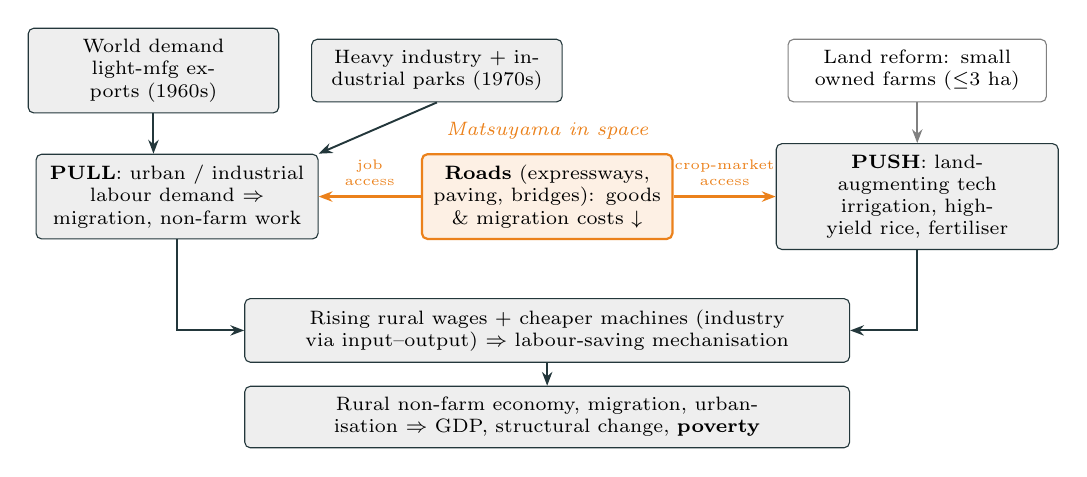
\begin{tikzpicture}
    \node[box=2.9cm] (wd) at (-5.0,0) {World demand\\light-mfg exports (1960s)};
    \node[box=2.9cm] (hci) at (-1.4,0) {Heavy industry + industrial parks (1970s)};
    \node[box=3.3cm] (pull) at (-4.7,-1.6)
      {\textbf{PULL}: urban / industrial labour demand $\Rightarrow$ migration, non-farm work};
    \node[box=2.9cm, hot] (roads) at (0,-1.6)
      {\textbf{Roads} (expressways, paving, bridges): goods \& migration costs $\downarrow$};
    \node[box=3.3cm] (push) at (4.7,-1.6)
      {\textbf{PUSH}: land-augmenting tech\\irrigation, high-yield rice, fertiliser};
    \node[box=3.0cm, draw=gray, fill=white] (lr) at (4.7,0)
      {Land reform: small owned farms ($\le$3 ha)};
    \node[box=7.4cm] (mech) at (0,-3.3) {Rising rural wages + cheaper machines (industry
      via input--output) $\Rightarrow$ labour-saving mechanisation};
    \node[box=7.4cm] (agg) at (0,-4.4) {Rural non-farm economy, migration, urbanisation
      $\Rightarrow$ GDP, structural change, \textbf{poverty}};
    \draw[arr] (wd.south) -- (wd.south |- pull.north);
    \draw[arr] (hci.south) -- (pull.north east);
    \draw[arr, mOrange, line width=1pt] (roads) -- node[above, font=\tiny, text=mOrange,
      align=center] {job\\access} (pull);
    \draw[arr, mOrange, line width=1pt] (roads) -- node[above, font=\tiny, text=mOrange,
      align=center] {crop-market\\access} (push);
    \draw[arr, gray] (lr) -- (push);
    \draw[arr] (pull.south) |- (mech.west);
    \draw[arr] (push.south) |- (mech.east);
    \draw[arr] (mech) -- (agg);
    \node[font=\scriptsize\itshape, text=mOrange, above=0.5mm of roads]
      {Matsuyama in space};
  \end{tikzpicture}
\end{frame}

\begin{frame}{A township in one equation}
  Competitive farms, $Q_i=(B_iT_i)^{\alpha}L_{Ai}^{1-\alpha}$; land-augmenting shock $B_i$
  (e.g.\ a reservoir). Local crop demand faced with elasticity $e_i$; opportunity wage $w_i$.
  \begin{equation*}
    d\log L_{Ai}
    \;=\;
    \frac{\overbrace{\alpha\,(e_i-1)\,d\log B_i}^{\text{commercialisation vs.\ food problem}}
          \;-\;\overbrace{e_i\,d\log w_i}^{\text{labour release}}}
         {\alpha e_i + 1-\alpha}
  \end{equation*}
  \begin{columns}[T]
    \begin{column}{0.52\textwidth}
      \footnotesize
      \begin{itemize}
        \item \textbf{Crop-market access} raises $e_i$: isolated $\approx$ local food
              demand elasticity ($<1$); connected $\to$ trade elasticity $\theta$ ($\gg1$).
        \item \textbf{Job access} moves $w_i$: industrial pull, migration.
        \item Fixed $w$: labour retained iff $e_i>1$ --- Matsuyama's two regimes as two ends
              of the access distribution.
        \item Connected places also respond \emph{more} to the opportunity wage.
      \end{itemize}
    \end{column}
    \begin{column}{0.44\textwidth}
      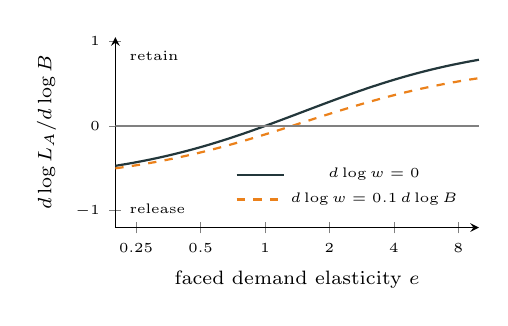
\begin{tikzpicture}
        \begin{axis}[width=6.2cm, height=4.0cm, xmode=log, xmin=0.2, xmax=10,
            ymin=-1.2, ymax=1.05, axis lines=left,
            xlabel={\scriptsize faced demand elasticity $e$},
            ylabel={\scriptsize $d\log L_A/d\log B$},
            tick label style={font=\tiny}, label style={font=\scriptsize},
            xtick={0.25,0.5,1,2,4,8}, xticklabels={0.25,0.5,1,2,4,8},
            legend style={font=\tiny, draw=none, at={(0.98,0.05)}, anchor=south east}]
          \addplot[domain=0.2:10, samples=120, mDarkTeal, thick]
            {0.4*(x-1)/(0.4*x+0.6)};
          \addlegendentry{$d\log w=0$}
          \addplot[domain=0.2:10, samples=120, mOrange, thick, dashed]
            {(0.4*(x-1)-0.1*x)/(0.4*x+0.6)};
          \addlegendentry{$d\log w=0.1\,d\log B$}
          \draw[gray, thin] (axis cs:0.2,0) -- (axis cs:10,0);
          \node[font=\tiny, anchor=north west] at (axis cs:0.21,1.0) {retain};
          \node[font=\tiny, anchor=south west] at (axis cs:0.21,-1.15) {release};
        \end{axis}
      \end{tikzpicture}\\
      \tiny Illustrative, $\alpha=0.4$; derivation in backup.
    \end{column}
  \end{columns}
\end{frame}

\begin{frame}{What the sign can and cannot tell us}
  \footnotesize
  A tempting test: ``the effect of irrigation on farm employment flips sign with market
  access''. Three reasons it is not, by itself, informative:
  \begin{enumerate}
    \item \textbf{Gravity builds in the flip.} With CES trade, connected places face
          $e=\theta>1$ and isolated places $e<1$. The data identify \hl{where} on the
          access distribution the crossing occurs --- which disciplines trade costs and
          Engel curves.
    \item \textbf{Connectivity moves both terms.} Better-connected townships also have
          non-farm jobs, cheaper machines and lower migration costs, which push towards
          release. We need \hl{separate} measures of crop-market and job access.
    \item \textbf{Irrigation is not Hicks-neutral.} Paddy irrigation and high-yield rice
          raised labour per hectare (double cropping, transplanting). The factor bias must
          be estimated jointly.
  \end{enumerate}
  \begin{exampleblock}{Our approach}
    \footnotesize
    The model, with trade, migration and Engel parameters estimated from other moments,
    \hl{predicts} the interaction coefficient; the township event studies estimate it. A
    held-out test. Township retention is also not aggregate retardation, so the
    aggregate consequences come from general equilibrium.
  \end{exampleblock}
\end{frame}

\begin{frame}{Labour-saving technology: mechanisation}
  A tiller cuts labour per hectare by a fraction $\chi$ and costs $u_t=p_{m,t}(r_t+d)$ a
  year. A farm of size $\ell$ adopts iff
  \begin{equation*}
    \chi\,\lambda_0\,\ell\,w_{iA,t}\;\ge\;u_t
    \quad\Longleftrightarrow\quad
    \ell\;\ge\;\ell^{*}_{it}=\frac{p_{m,t}\,(r_t+d)}{\chi\,\lambda_0\,w_{iA,t}},
    \qquad
    \text{adoption}_{it}=1-F_i\bigl(\ell^{*}_{it}\bigr).
  \end{equation*}
  \begin{columns}[T]
    \begin{column}{0.55\textwidth}
      \small
      \begin{itemize}
        \item $F_i$: observed landholding distribution, a legacy of land reform.
        \item Adoption responds to farm wages (\hl{industrial pull}), machine prices
              (\hl{domestic machinery industry} via input--output), and farm size.
        \item Induced innovation (Hayami--Ruttan) with a micro-founded extensive margin.
      \end{itemize}
    \end{column}
    \begin{column}{0.41\textwidth}
      \begin{block}{Why it matters}
        \small
        Labour-saving change \hl{releases} labour; land-augmenting change can
        \hl{absorb} it (Bustos--Caprettini--Ponticelli 2016). Korea had both, in different
        places and at different times.
      \end{block}
    \end{column}
  \end{columns}
\end{frame}

% =====================================================================
\section{Model}
% =====================================================================

\begin{frame}{Environment}
  \begin{columns}[T]
    \begin{column}{0.5\textwidth}
      \small
      Sequence of spatial equilibria; state = lagged population.
      \begin{itemize}
        \item Locations $d\in\mathcal N$; current quantification: five (Seoul, Busan,
              Changwon, Daegu, rural Korea).
        \item \textbf{Four sectors}:
          \begin{itemize}\footnotesize
            \item \textbf{Rice}: protected, internationally non-traded; can be mechanised.
            \item \textbf{Other agriculture}: competes with imports at world prices.
            \item \textbf{Manufacturing}: traded; the export sector.
            \item \textbf{Services}: non-traded.
          \end{itemize}
        \item Input--output linkages; trade costs between locations; sector-specific
              agglomeration.
      \end{itemize}
    \end{column}
    \begin{column}{0.46\textwidth}
      \small
      \begin{itemize}
        \item Non-homothetic (PIGL) demand.
        \item Migration across locations, nested with occupation choice within them.
        \item Heterogeneous producers; farms select into mechanisation.
        \item Local land ownership; government spending buys output.
        \item Small open economy; trade balance pinned to an exogenous path.
        \item Growth: sectoral TFP growth and rising foreign demand for manufactures.
      \end{itemize}
    \end{column}
  \end{columns}
\end{frame}

\begin{frame}{Preferences: the food problem}
  PIGL indirect utility (Boppart 2014) at income $y$ and prices $P_{dj}$,
  $\mathcal P_d=\prod_jP_{dj}^{\alpha_j}$:
  \begin{equation*}
    V_d=\frac1\eta\Bigl(\frac{y}{\mathcal P_d}\Bigr)^{\eta}-\sum_j v_j\log P_{dj},
    \qquad
    \psi_{dj}=\alpha_j+v_j\Bigl(\frac{y}{\mathcal P_d}\Bigr)^{-\eta},
    \qquad \textstyle\sum_j\alpha_j=1,\ \sum_jv_j=0.
  \end{equation*}
  \small
  \begin{itemize}
    \item $\eta>0$, $v_{\text{food}}>0$: the food share falls with real income; the
          services share rises.
    \item Aggregates exactly over finitely many income groups: farm and non-farm
          households demand different baskets, so the \emph{composition} of local income
          shapes local demand (rural services).
    \item Migration and welfare use the money-metric equivalent income
          $\mathcal Y=\mathcal P_0[\eta(V+z_0)]^{1/\eta}$, so choices and welfare rank
          places exactly as utility does.
  \end{itemize}
\end{frame}

\begin{frame}{Location $\times$ occupation choice}
  Agent in origin $o$ chooses location $d$ and occupation $\kappa\in\{$farm, manufacturing,
  services$\}$ to maximise
  $W_{od}+\log b_{d\kappa}+\log\mathcal Y_{d\kappa}+\upsilon_{i,d\kappa}$, with nested-logit
  (GEV) shocks:
  \begin{equation*}
    \pi_{\kappa\mid d}=\frac{(b_{d\kappa}\mathcal Y_{d\kappa})^{\varepsilon}}
                            {\sum_{\kappa'}(b_{d\kappa'}\mathcal Y_{d\kappa'})^{\varepsilon}},
    \qquad
    \Phi_d=\Bigl[\sum_\kappa(b_{d\kappa}\mathcal Y_{d\kappa})^{\varepsilon}\Bigr]^{1/\varepsilon},
    \qquad
    \mu_{od}\propto\Bigl(\frac{\bar V_d\,L_{d,t-1}^{\iota}\,\Phi_d}{\delta_{od}}\Bigr)^{\nu}.
  \end{equation*}
  \small
  \begin{itemize}
    \item $\nu\le\varepsilon$: switching sector within a place is easier than moving.
    \item $b_{d\kappa}$: non-pecuniary value of an occupation --- attachment to farming,
          barriers to leaving it.
    \item Each location--occupation labour market clears at its own wage.
    \item Welfare by origin is the inclusive value;
          $\partial\,\mathbb E U_o/\partial\log\mathcal Y_{d\kappa}=\mu_{od}\pi_{\kappa\mid d}$.
    \item Limit $\varepsilon\to\infty$, $b=1$: one integrated wage per location.
  \end{itemize}
\end{frame}

\begin{frame}{Why sectoral wages: the agricultural productivity gap}
  With one wage per location, farm and non-farm value added per worker differ only through
  labour shares $\lambda^k$:
  \begin{equation*}
    \mathrm{APG}_d\equiv\frac{\mathrm{VA}^A_d/L^A_d}{\mathrm{VA}^N_d/L^N_d}
    =\frac{w^A_d/\lambda^A_d}{w^N_d/\lambda^N_d}
    \;\overset{w^A=w^N}{=}\;\frac{\lambda^N_d}{\lambda^A_d}\;\gtrsim 1,
  \end{equation*}
  far from the gaps measured in poor economies (Gollin--Lagakos--Waugh 2014).
  \begin{block}{Wage-gap decomposition}
    \vspace{-0.6em}
    \begin{equation*}
      \log\frac{\mathcal Y_{dA}}{\mathcal Y_{dN}}
      =\underbrace{\frac1\varepsilon\log\frac{L_{dA}}{L_{dN}}}_{\text{finite supply elasticity}}
      \;-\;\underbrace{\log\frac{b_{dA}}{b_{dN}}}_{\text{non-pecuniary wedge}}
    \end{equation*}
  \end{block}
  \footnotesize
  \begin{itemize}
    \item A large farm share at a \emph{lower} farm wage requires $b_A>b_N$.
    \item When farm labour demand falls, finite $\varepsilon$ keeps workers in farming at a
          falling relative wage: the gap \hl{widens} before switching and migration catch
          up.
  \end{itemize}
\end{frame}

\begin{frame}{Production, trade and equilibrium}
  \small
  \begin{itemize}
    \item \textbf{Producers}: monopolistic competition with productivity draws; entry,
          exporting and (in rice) mechanisation are a nested discrete choice --- only active
          producers mechanise or export.
    \item \textbf{Mechanisation} substitutes machinery for labour. Its profit gain
          \begin{equation*}
            \Delta=\Bigl(\xi\,\frac{c}{\breve c}\Bigr)^{\sigma-1}-1
          \end{equation*}
          rises with $w/P_{\text{machinery}}$: adoption turns on as \hl{wages rise and
          machines get cheaper}.
    \item \textbf{Trade}: CES across origins with iceberg costs; foreign varieties at
          world prices; aggregate export demand elasticity $\sigma_x$. External balance
          $\mathrm{EX}-\mathrm{IM}=\mathrm{NX}^\star_t$ pins the domestic price level.
    \item \textbf{Equilibrium}: migration and occupation shares, PIGL demand, firm choices,
          goods, labour and land market clearing, government budget, external balance.
          Solved as a fixed point; adding-up holds to machine precision.
    \item \textbf{Initial condition}: 1965 amenities inverted so the observed 1965
          population is an equilibrium; urbanisation after 1965 is a \hl{model outcome}.
  \end{itemize}
\end{frame}

% =====================================================================
\section{Quantification (preliminary)}
% =====================================================================

\begin{frame}{Calibrating to history: 8 parameters, 8 targets}
  \begin{columns}[T]
    \begin{column}{0.6\textwidth}
      \scriptsize
      \begin{tabular}{@{}lll@{}}
        \toprule
        Parameter & Value & Main target \\
        \midrule
        Manufacturing TFP growth & 4.1\%/yr & real GDP p.c., 1985/65 \\
        Farm and services TFP growth & 3.2\%/yr & mfg VA share 1985 \\
        PIGL income elasticity $\eta$ & 0.39 & farm emp.\ share 1985 \\
        PIGL food shifter $v_{\text{food}}$ & 0.51 & farm emp.\ share 1965 \\
        Mfg weight in non-food demand & 0.02 & mfg VA share 1965 \\
        Foreign demand, 1965 level & --- & exports/GDP 1965 \\
        Foreign demand growth & 24\%/yr & exports/GDP 1985 \\
        Urban non-farm TFP premium & 1.17 & urban share 1980 \\
        \bottomrule
      \end{tabular}\\[0.3em]
      \tiny Exactly identified; the 1965 amenity inversion is redone at every evaluation.
    \end{column}
    \begin{column}{0.36\textwidth}
      \footnotesize
      \textbf{Set externally}: $\sigma=4$, Pareto shape 5, migration elasticity
      $\nu=5$, mechanisation gain $\xi=1.2$, land shares, input--output coefficients,
      trade and migration costs.\\[0.5em]
      \textbf{Current simplifications}: five stylised regions; six periods
      (1965--85); rice half of food demand; stylised input--output table.
    \end{column}
  \end{columns}
\end{frame}

\begin{frame}{The baseline reproduces Korea's transformation}
  \centering
  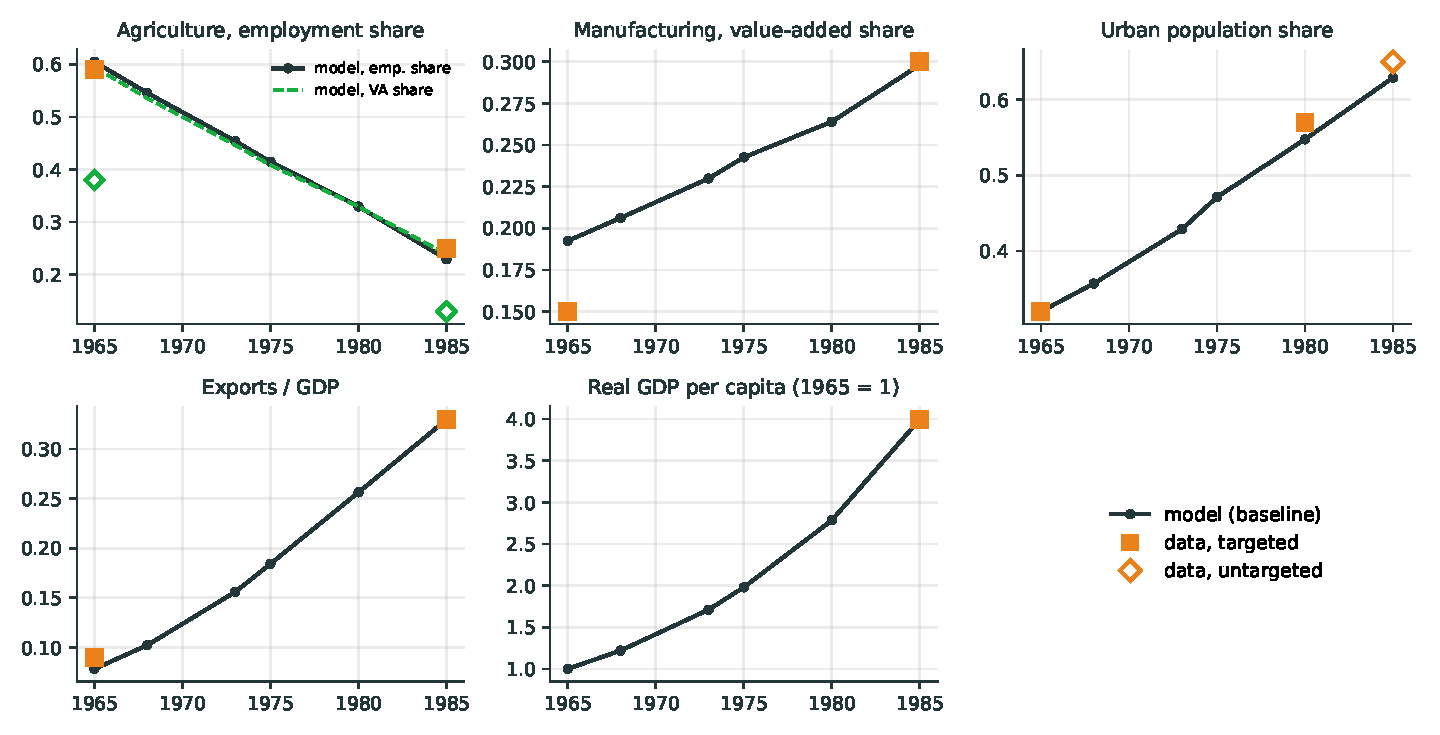
\includegraphics[width=0.9\textwidth]{fig_history_fit_conf.pdf}\\
  \scriptsize Green: farm value-added share (model dashed; data hollow). Several data
  targets are approximate and being updated from primary sources.
\end{frame}

\begin{frame}{What drives it, and where it misses}
  \begin{columns}[T]
    \begin{column}{0.5\textwidth}
      \textbf{Accounting for the transformation}
      \begin{itemize}\small
        \item Farm employment falls 38 points (0.61 $\to$ 0.23) through \hl{Engel effects}
              on rising income, \hl{grain import competition} (import share of other farm
              demand 0.10 $\to$ 0.76) and \hl{migration}.
        \item Urbanisation 0.32 $\to$ 0.63 is generated, not imposed (1985 untargeted:
              0.63 vs 0.65).
        \item Export share 8\% $\to$ 33\% requires foreign demand for manufactures growing
              $\sim$24\%/yr.
        \item Rice mechanisation takes off only after the mid-1970s, as wages rise.
      \end{itemize}
    \end{column}
    \begin{column}{0.46\textwidth}
      \textbf{Where it misses}
      \begin{itemize}\small
        \item \hl{No productivity gap} with integrated local labour markets: 1965 farm VA
              share 0.60 vs $\approx$0.38 in the data $\Rightarrow$ occupation wedges
              (next slide).
        \item 1965 manufacturing share too high (0.19 vs 0.15): stylised input--output
              structure $\Rightarrow$ Korean IO tables.
        \item No relative-price (Baumol) channel in demand.
      \end{itemize}
    \end{column}
  \end{columns}
\end{frame}

\begin{frame}{Occupation wedges open --- and widen --- the productivity gap}
  \footnotesize
  \centering
  \begin{tabular}{@{}lcccccc@{}}
    \toprule
    & \multicolumn{3}{c}{1965} & \multicolumn{3}{c}{1985} \\
    \cmidrule(lr){2-4}\cmidrule(lr){5-7}
    & farm emp. & $w_A/w_N$ & APG & farm emp. & $w_A/w_N$ & APG \\
    \midrule
    integrated ($\varepsilon=\infty$) & 0.605 & 0.827 & 0.958 & 0.229 & 0.868 & 1.053 \\
    $\varepsilon=5$, $b_A=1$ & 0.530 & 1.051 & 1.214 & 0.218 & 0.908 & 1.107 \\
    $\varepsilon=5$, $b_A=1.5$ & 0.627 & 0.802 & 0.930 & 0.314 & 0.676 & 0.803 \\
    $\varepsilon=5$, $b_A=2$ & 0.680 & 0.653 & \hl{0.758} & 0.399 & 0.545 & \hl{0.638} \\
    \bottomrule
  \end{tabular}\\[0.2em]
  \tiny Comparative statics: 1965 amenities re-inverted per case, other parameters at the
  integrated calibration (not yet recalibrated). APG = farm VA per worker / non-farm.
  \vspace{0.5em}
  \begin{enumerate}\small
    \item $b_A=1$ is \emph{not} frictionless: equal pay would mean equal occupation shares,
          so a large farm share needs a higher farm wage.
    \item With a farm wedge the gap \hl{appears and widens} during the transformation
          (APG 0.76 $\to$ 0.64): falling farm labour demand lowers the farm wage faster than
          workers leave.
    \item The wedge also \hl{slows} the transformation. Separating $b_A$, $\varepsilon$ and
          the Engel parameters requires farm and non-farm earnings data.
  \end{enumerate}
\end{frame}

% =====================================================================
\section{Data and empirical strategy}
% =====================================================================

\begin{frame}{A new township panel, 1960--90}
  \small
  Annual township-level data being digitised from statistical yearbooks:
  \vspace{0.3em}

  \footnotesize
  \begin{tabular}{@{}L{0.24\textwidth}L{0.42\textwidth}L{0.26\textwidth}@{}}
    \toprule
    Block & Variables & Role in the model \\
    \midrule
    Population & population; employed / unemployed / inactive; employment by sector &
      amenities, occupation shares, non-employment \\
    Agriculture & land by type (paddy / dry); farm households by landholding size;
      reservoirs (capacity, date); crops, livestock & farm-size distribution; irrigation
      shock; crop mix \\
    Infrastructure & roads paved / unpaved; bridges; ports; electricity &
      local access; dated shocks \\
    Municipal finance & revenue, central transfers, spending by function &
      local public investment \\
    Schools & schools, students, teachers, enrolment & human capital \\
    \bottomrule
  \end{tabular}
  \vspace{0.4em}

  \small Complemented by county manufacturing surveys, the digitised road network
  (1967/75/87), and national accounts.
\end{frame}

\begin{frame}{Testing the mechanism: reservoirs}
  \small
  \begin{columns}[T]
    \begin{column}{0.5\textwidth}
      \begin{itemize}
        \item Event studies of reservoir completions, heterogeneous by \hl{predetermined}
              access to \emph{crop markets} and, separately, to \emph{non-farm employment}.
        \item Treatment follows the irrigation \emph{command area}, not the township
              containing the dam.
        \item Placebo: dry-field townships.
        \item Outcome: farm employment \emph{share} (migration contaminates levels).
        \item A reversal requires the effect to \hl{cross zero} within the observed
              support of access.
      \end{itemize}
    \end{column}
    \begin{column}{0.46\textwidth}
      \footnotesize
      \begin{tabular}{@{}L{0.3\textwidth}L{0.62\textwidth}@{}}
        \toprule
        Channel & Evidence \\
        \midrule
        Commercia\-lisation & marketed output, farm-gate prices, farm labour demand,
          land returns \\
        Labour release & labour per hectare $\downarrow$, mechanisation, non-farm work,
          migration \\
        Local demand spillovers & rural services after farm-income gains \\
        \bottomrule
      \end{tabular}\\[0.4em]
      \small Model side: the predicted interaction coefficient, with trade, migration and
      Engel parameters set from other moments.
    \end{column}
  \end{columns}
\end{frame}

\begin{frame}{From township estimates to aggregate effects}
  \small
  Township designs identify \emph{relative} effects; year effects absorb national prices,
  migration to cities and fiscal costs. The model supplies the general-equilibrium
  \hl{intercept}.
  \vspace{0.3em}

  \footnotesize
  \begin{tabular}{@{}L{0.33\textwidth}L{0.6\textwidth}@{}}
    \toprule
    Parameter & Identified from \\
    \midrule
    Trade elasticity, distance cost & price gaps across markets; market-access event studies \\
    Migration elasticity and costs & origin--destination flows; expressway interchange openings \\
    Occupation elasticity $\varepsilon$, wedges $b$ & sectoral employment responses to
      shift-share industrial demand; earnings gaps \\
    Engel parameters & household-survey Engel curves \\
    Mechanisation threshold & adoption by farm-size class $\times$ wage and machine-price shocks \\
    Irrigation factor bias & reservoir event studies; labour per hectare \\
    \bottomrule
  \end{tabular}
  \vspace{0.4em}

  \small
  \textbf{Counterfactuals}: subtract measured shocks from history and decompose growth,
  structural change and \hl{poverty} across drivers (world demand, industrial policy,
  roads, rural programmes) with Shapley values; price complementarities such as
  parks $\times$ roads.
\end{frame}

\begin{frame}{Summary and next steps}
  \begin{block}{Summary}
    \small
    \begin{itemize}
      \item Whether farm productivity growth retains or releases labour depends on two
            access margins --- to crop markets and to non-farm jobs --- which
            connectivity moves together.
      \item Korea's closed-but-integrated rice market makes the Matsuyama regime a
            township-level variable.
      \item A spatial GE model calibrated to history reproduces the 1965--85
            transformation; occupation wedges deliver a widening productivity gap.
    \end{itemize}
  \end{block}
  \textbf{Next}
  \begin{itemize}\footnotesize
    \item A township-level spatial model with competitive farms on paddy and dry land,
          irrigation as a factor-biased shock, and the observed farm-size distribution.
    \item Reservoir and road-paving event studies on the township panel.
    \item Recalibrate with sectoral earnings and Korean input--output tables; annual
          clock; capital and schooling for the aggregate decomposition.
  \end{itemize}
\end{frame}

\begin{frame}[standout]
  Thank you\\[0.6em]
  \normalsize Comments very welcome\\
  \small [email]
\end{frame}

% =====================================================================
\appendix
\metroset{sectionpage=none}
\section{Backup}
% =====================================================================

\begin{frame}{Backup: derivation of the township equation}
  \small
  Competitive farm, Cobb--Douglas: $p(1-\alpha)Q/L_A=w$ with $Q=(BT)^\alpha L_A^{1-\alpha}$
  gives
  \begin{equation*}
    \log L_A=\tfrac1\alpha\bigl[\log(1-\alpha)+\log p+\alpha\log(BT)-\log w\bigr].
  \end{equation*}
  Faced demand $Q=D\,p^{-e}$, so $d\log p=-\frac1e\,d\log Q=-\frac1e[\alpha\,d\log B+(1-\alpha)\,d\log L_A]$.
  Substituting and collecting $d\log L_A$:
  \begin{equation*}
    d\log L_A\Bigl(\alpha+\frac{1-\alpha}{e}\Bigr)=\alpha\Bigl(1-\frac1e\Bigr)d\log B-d\log w
    \;\Longrightarrow\;
    d\log L_A=\frac{\alpha(e-1)\,d\log B-e\,d\log w}{\alpha e+1-\alpha}.
  \end{equation*}
  \begin{itemize}
    \item $e\to\infty$ (price-taker): $d\log L_A=d\log B-\frac1\alpha d\log w$.
    \item Partial equilibrium and Hicks-neutral; the quantitative model endogenises $e$
          and $w$ and allows factor bias.
  \end{itemize}
\end{frame}

\begin{frame}{Backup: nested entry, adoption and export}
  \small
  With $x=\phi^{\sigma-1}$, every option's profit is linear in $x$: option $k$ has slope
  $a_k$ and fixed cost $c_k$. Rice: exit $(0,0)$, traditional $(a^T,F)$, mechanised
  $(a^M,F+\breve F)$, mechanised exporter $(a^M+a^X,F+\breve F+\tilde F)$. The producer
  picks the upper envelope:
  \begin{equation*}
    \text{``option }k\text{ or higher''}\iff x\ge X_k,\qquad
    X_k=\min_{k'\ge k}\;\max_{i<k'}\frac{c_{k'}-c_i}{a_{k'}-a_i}.
  \end{equation*}
  A traditional segment exists iff
  \begin{equation*}
    \frac{\breve F}{F}>\Delta,\qquad
    \frac{\breve F+\tilde F}{F}>\Delta+\frac{a^X}{a^T},\qquad
    \Delta\equiv\Bigl(\xi\,\frac{c}{\breve c}\Bigr)^{\sigma-1}-1 .
  \end{equation*}
  Fixed costs are in units of local labour, so they rise with wages. In the planned
  township model this block is replaced by competitive farms with the farm-size threshold.
\end{frame}

\begin{frame}{Backup: decomposition and poverty}
  \small
  \textbf{Shapley decomposition} over drivers $D$ (world demand, capital, human capital,
  demography, industrial credit, parks, roads, rural programmes, residual TFP):
  \begin{equation*}
    \phi_d=\sum_{S\subseteq D\setminus\{d\}}\frac{|S|!\,(|D|-|S|-1)!}{|D|!}\,
    \bigl[Y(S\cup\{d\})-Y(S)\bigr].
  \end{equation*}
  Pairwise complementarity: $Y(a,b)-Y(a)-Y(b)+Y(\varnothing)$.\\[0.5em]
  \textbf{Poverty} from model incomes by (location, occupation, land class) with
  within-cell lognormal dispersion $\sigma_c$ from household surveys:
  \begin{equation*}
    H_t=\sum_c\omega_{c,t}\,\Phi\Bigl(\frac{\ln z-\ln\bar y_{c,t}}{\sigma_c}+\frac{\sigma_c}{2}\Bigr).
  \end{equation*}
\end{frame}

\begin{frame}{References}
  \begin{columns}[T]
    \begin{column}{0.48\textwidth}
    \scriptsize
    \begin{itemize}\setlength{\itemsep}{0pt}
      \item Adão, Arkolakis \& Esposito (2019) General equilibrium effects in space
      \item Allen \& Arkolakis (2014, QJE)
      \item Boppart (2014, ECMA)
      \item Budí-Ors \& Pijoan-Mas (WP) Rural exodus and uneven industrialisation
      \item Buera, Kaboski \& Townsend (2023, JEL)
      \item Bustos, Caprettini \& Ponticelli (2016, AER)
      \item Cheung \& Yang (2024, WP) Transportation networks, technology adoption, and
            structural transformation
      \item Donaldson (2018, AER)
      \item Eckert \& Peters (WP) Spatial structural change
      \item Fan, Peters \& Zilibotti (2023, ECMA)
      \item Foster \& Rosenzweig (2004, EDCC)
      \item Gollin, Lagakos \& Waugh (2014, QJE)
      \item Gollin, Parente \& Rogerson (2007, JME)
      \item Gollin \& Rogerson (2014, JDE)
      \item Hao, Sun, Tombe \& Zhang (2020) The geography of development
    \end{itemize}
    \end{column}
    \begin{column}{0.48\textwidth}
    \scriptsize
    \begin{itemize}\setlength{\itemsep}{0pt}
      \item Hayami \& Ruttan (1971)
      \item Hsieh, Hurst, Jones \& Klenow (2019, ECMA)
      \item Lagakos \& Waugh (2013, AER)
      \item Lagakos, Mobarak \& Waugh (2023, ECMA)
      \item Matsuyama (1992, JET) Agricultural productivity, comparative advantage, and
            economic growth
      \item Nakamura \& Steinsson (2018, JEP)
      \item Redding \& Rossi-Hansberg (2017, ARE)
      \item Sotelo (2020, JPE)
      \item Teignier (2018, JDE)
      \item Tombe \& Zhu (2019, AER)
      \item Uy, Yi \& Zhang (2013, JME)
    \end{itemize}
    \end{column}
  \end{columns}
\end{frame}

\end{document}
